\section{Evaulation}
\label{sec-evaluation}

%Metrics: what do you care about?
%Evaluation methodology: how did you evaluate?
%Results / discussions: if possible, provide intuitions and reasons for the
%result you got.

As described in the previous section, our study focuses on analyzing the AC and
DC power consumption ratios.

\begin{table}[!htb]
  \centering
    \begin{tabular}{| c | c |}
      \hline
      \textbf{DBI Ratio} & \textbf{Improvement \%} \\ \hline
     Load DC  & 68.59 \\ \hline
     Load AC  & 8.62  \\ \hline
     Store DC & 75.04 \\ \hline
     Store AC & 3.38  \\ \hline
    \end{tabular}
    \caption{AC/DC ratio reduction for load and store operations using DBI}
    \label{table:dbi-ratios}
\end{table}

\begin{figure}[!htb]
  \centering
  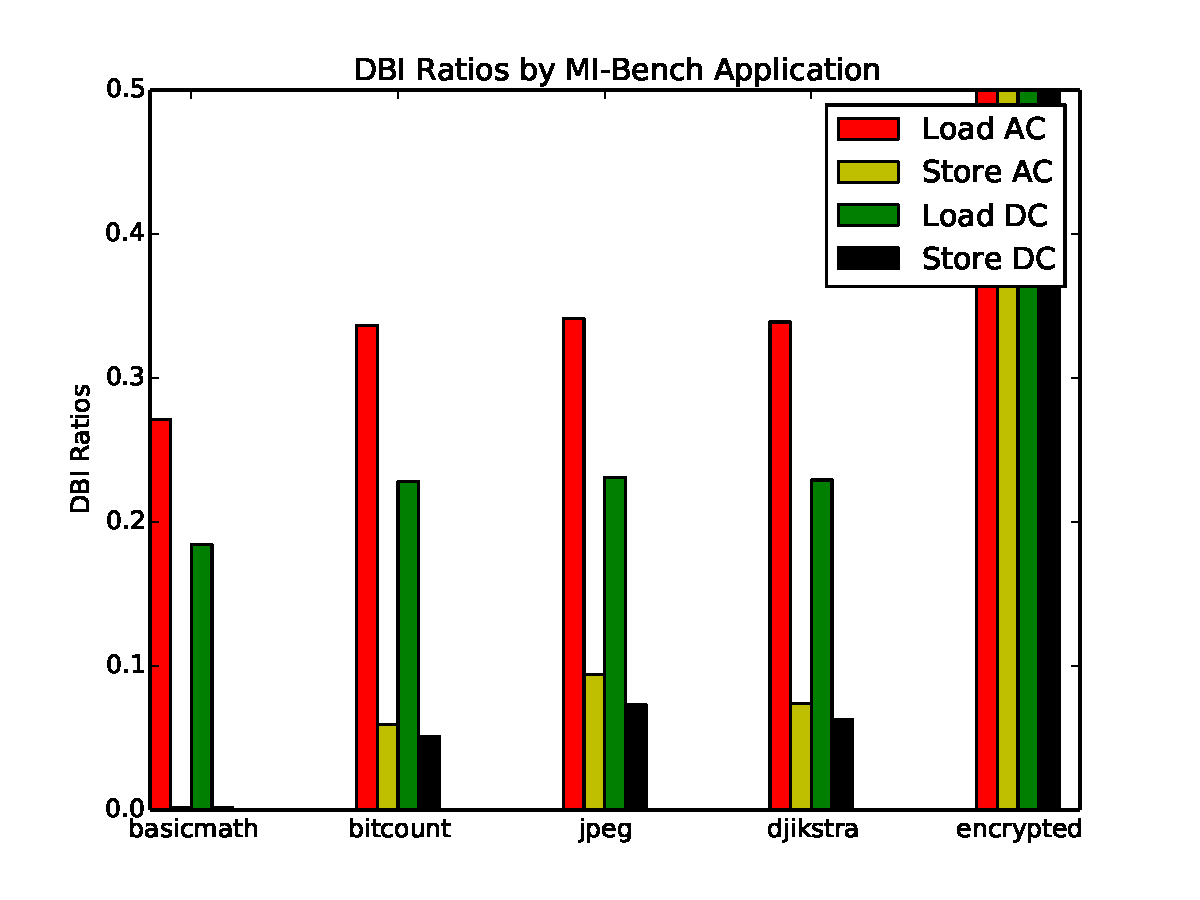
\includegraphics[width=0.5\textwidth]{figs/dbiGraph}
  \caption{Comparing load/store DBI ratios for representative MiBench applications}
  \label{fig:dbiGraph}
\end{figure}

\begin{enumerate}
  \item Looking at A, B ratios for loads and stores.
  \item Put graphs and analyze them.
  \item Intuition for decrease (store is lower - mostly misses)
\end{enumerate}

